\chapter{Release 2: Sending notifications \& dashboards}

\phantomsection
\section*{Introduction}
\addcontentsline{toc}{section}{Introduction}
Throughout this chapter, we will delve into the planning, design considerations, and implementation of our
second product release. Building upon the foundation laid in our initial release, our focus now shifts
towards fine-tuning the intricacies of notifications. This release encompasses a comprehensive overhaul
of the notification system, spanning key areas such as notification templates, user preferences, delivery
triggers, notification history, and the development of a powerful dashboard to provide insights into
the delivery of notifications.

\section{Sprint backlog}
During the second sprint planning event, we estimated the effort required for each item in the third and
fourth sprints backlog based on the number of working hours. The priority of backlog items is reflected
by their relative order in the table, same as the first release, items positioned higher in the table
indicate a higher priority. \\

\begin{longtable}{ | m{0.08\textwidth}  | m{0.18\textwidth} | m{0.39\textwidth} | c | }
    \caption{Backlog of Sprint 3 \& 4}                                                                                                          \\
    \hline
    \textbf{Sprint}         & \textbf{Epic}                                        & \textbf{User story}          & \textbf{Estimation (hours)} \\
    \hline
    \endfirsthead
    \hline
    \textbf{Sprint}         & \textbf{Epic}                                        & \textbf{User story}          & \textbf{Estimation (hours)} \\
    \hline
    \endhead
    \hline
    \endfoot
    \endlastfoot
    \multirow[t]{2}{5em}{3} & \multirow{4}{5em}{Notification templates management} & Create a template            & 24                          \\
    \cline{3-4}
                            &                                                      & List templates               & 16                          \\
    \cline{3-4}
                            &                                                      & Edit a template              & 8                           \\
    \cline{3-4}
                            &                                                      & Delete a template            & 8                           \\
                            & Notification preferences management                  & Set notification preferences & 16                          \\
    \hline
    \multirow[t]{2}{5em}{4} & \multirow{4}{5em}{Notification triggers management}  & Create a trigger             & 48                          \\
    \cline{3-4}
                            &                                                      & List triggers                & 16                          \\
    \cline{3-4}
                            &                                                      & Edit a trigger               & 8                           \\
    \cline{3-4}
                            &                                                      & Delete a trigger             & 8                           \\
    \cline{2-4}
                            & \multirow{2}{5em}{Notification history}              & Get notification history     & 24                          \\
    \cline{3-4}
                            &                                                      & List sending logs            & 16                          \\
    \cline{2-4}
                            & Dashboard                                            & View metrics                 & 32                          \\
    \hline
\end{longtable}

\section{Specification}
Similar to our approach in the first release, we will be detailing some selected user stories that
we find most significant to drive the enhancements planned for this release.

\begin{longtable}{ | m{0.2\textwidth} | m{0.75\textwidth} | }
    \caption{User stories specification for the second release}                                                                                                                                                                                  \\
    \hline
    \textbf{Epic}                                       & \textbf{User story}                                                                                                                                                                    \\
    \hline
    \endfirsthead
    \hline
    \textbf{Epic}                                       & \textbf{User story}                                                                                                                                                                    \\
    \hline
    \endhead
    \endfoot
    \endlastfoot
    Notification \newline templates \newline management & \textbf{Create a template} \newline As an agent, I want to be able to add notification templates so that I can send notifications based on that template.

    \paragraph*{Precondition} \mbox{} \newline
    \begin{itemize}
        \item Agent is authenticated and has a valid account.
        \item Existing notification topic.
    \end{itemize}

    \paragraph*{Business rules} \mbox{} \newline
    \begin{itemize}
        \item Notification templates should include a name, a topic, a channel type, and the notification content.
        \item Agents should be able to add placeholders for dynamic data in the template body.
        \item Agents should be able to preview and test notification templates before saving.
    \end{itemize}
    \paragraph*{Technical specification} \mbox{} \newline
    \begin{itemize}
        \item The system should persist notification templates in the database unpopulated with data.
        \item Agents should be able to preview the notification template with test data without actually sending
              the notification to ensure that the message is rendered correctly.
    \end{itemize}
    \paragraph*{Acceptance criteria} \mbox{} \newline
    \begin{itemize}
        \item Notification templates must have a name, a selected channel type, and non-empty body.
        \item Agents can to add placeholders for dynamic data in the notification body.
        \item Agents can preview the template with actual data and verify that the message is generated correctly.
        \item A message indicating the success or failure of the saving operation is displayed.
    \end{itemize}                                                                                                                                    \\
    \hline
    Notification \newline triggers \newline management  & \textbf{Create a trigger} \newline As an agent, I want to be able to create triggers for notifications so that I can schedule notifications to be sent automatically.
    \paragraph*{Precondition} \mbox{} \newline
    \begin{itemize}
        \item Agent authenticated and has a valid account.
        \item Existing notification templates.
        \item Existing audiences.

    \end{itemize}
    \paragraph*{Business rules} \mbox{} \newline
    \begin{itemize}
        \item Agents should be able to choose a specific notification template.
        \item Agents should be able to choose a specific audience to target.
        \item Agents should be able to choose a delivery type for the trigger, either one time or recurring delivery.
        \item Agents should be able to choose a frequency of sending notification in the recurring delivery type.
        \item Agents should be able to specify a starting and ending date for the recurring delivery type.
        \item Agents could create multiple triggers for the same notification template or audience.
    \end{itemize}
    \paragraph*{Technical specification} \mbox{} \newline
    \begin{itemize}
        \item The system should provide a form where agents can select a notification template, an audience,
              set the trigger's schedule, and save the trigger.
        \item The system should use a cron job or similar scheduling mechanism to send notifications
              according to the trigger's schedule.
        \item The system should store the trigger and its associated scheduling data in the database.
    \end{itemize}
    \paragraph*{Acceptance criteria} \mbox{} \newline
    \begin{itemize}
        \item Agents can sucessfully schedule the two types of notification delivery.
        \item The notification system sends the notification according to the trigger's schedule.
        \item The notification system stores the trigger and associated metadata in a database.
        \item A message indicating the success or failure of the scheduling operation is displayed.
    \end{itemize}                                                                                                                                                   \\
    \hline
    Dashboard                                           & \textbf{View metrics} \newline As an agent I want to be able to view metrics on my dashboard so that I can get an overview on important statistics related to notification activities.
    \paragraph*{Precondition} \mbox{} \newline
    \begin{itemize}
        \item Agent is authenticated and has a valid account.
    \end{itemize}
    \paragraph*{Business rules} \mbox{} \newline
    \begin{itemize}
        \item Administrators should be able to get a high-level metrics including: total number of sent
              notifications, subscriptions, delivery rates, open rates, and click-through rates.
        \item The agent should be able to get an overview of notification activity specific to his account.
        \item The administrator/agent should be able to get an overview on sent notifications by each of the
              channels to understand which ones are the most effective.
        \item The administrator/agent should be able to get an overview on sent notifications metrics by each
              of the created segments of recipients.
        \item The administrator/agent should be able to get an overview on sent notifications metrics by each
              of the created templates.
    \end{itemize}
    \paragraph*{Technical specification} \mbox{} \newline
    \begin{itemize}
        \item Overviews should be displayed in the form of charts providing the metric for the current day and previous days.
        \item Overviews by channel, audience or template should display the number of sent notifications per each category
              out of total.
        \item Old metrics should be cached so that the system does not recalculate them with every request.        .
        \item Actual metrics should be calculated in real-time with a defined interval of update.
    \end{itemize}
    \paragraph*{Acceptance criteria} \mbox{} \newline
    \begin{itemize}
        \item Overviews are displaying accurate metrics.
        \item Update is happening after every defined interval of time.
        \item Agents are getting metrics only for the notifications they sent.
        \item Agents are getting metrics only for the templates and segments they created.
    \end{itemize}                                                                                                                                                            \\
    \hline
\end{longtable}

\section{Design}
Building upon the insights gained from the initial design, this phase focuses on refining and expanding our
software's architecture. In this section, we will explore the key considerations, decisions, and advancements
made during this second release.

\subsection{Database design}
In this section, We will elaborate on the structure and organization of our database from the first release,
defining new tables and relationships for the implementation of this second release of our product.

\subsubsection{Data dictionary}
In the table \ref{tab-r2dd}, we provide a comprehensive overview of the essential data elements
that will define our entities and relationships for the second release.

\subsubsection{Logical data model}
Building upon the foundation laid in our initial logical data model, we enter a phase of refinement and
expansion. In this section, we present the second iteration of our logical data model, which encapsulates
the newly added entities during this second release. This updated data model will offer
deeper insights into the structure and relationships of our data entities for the whole solution.

\noindent The figure \ref{r2-erd} illustrates the updated entity-relationship diagram for this second release.

\begin{landscape}
    \begin{longtable}{ | m{0.225\textwidth} | m{0.28\textwidth} | m{0.55\textwidth} | m{0.15\textwidth} | m{0.2\textwidth} | }
        \caption{Data dictionary of the second release}   \label{tab-r2dd}                                                                                                                                                                  \\
        \hline
        \textbf{Entity}                                                  & \textbf{Field}                            & \textbf{Description}                                                 & \textbf{Type} & \textbf{Constraints}          \\
        \hline
        \endfirsthead
        \hline
        \textbf{Entity}                                                  & \textbf{Field}                            & \textbf{Description}                                                 & \textbf{Type} & \textbf{Constraints}          \\
        \hline
        \endhead
        \hline
        \endfoot
        \endlastfoot
        \multirow[t]{5}{5em}{\textbf{Topic}}                             & \texttt{id}                               & Topic's unique identifier                                            & bigint        & Primary key \newline Not null \\
        \cline{2-5}
                                                                         & \texttt{name}                             & Topic's name                                                         & varchar(100)  & Unique, Not null              \\
        \cline{2-5}
                                                                         & \texttt{description}                      & Topic's description                                                  & varchar(256)  &                               \\
        \cline{2-5}
                                                                         & \texttt{priority}                         & Topic's notification sending priority                                & varchar(10)   & Not null                      \\
        \cline{2-5}
                                                                         & \texttt{creator\char`_id}                 & Topic's creator unique identifier                                    & bigint        & Not null                      \\
        \hline
        \multirow[t]{8}{5em}{\textbf{Template}}                          & \texttt{id}                               & Notification template's unique identifier                            & bigint        & Primary key \newline Not null \\
        \cline{2-5}
                                                                         & \texttt{name}                             & Notification template's unique name                                  & varchar(100)  & Not null                      \\
        \cline{2-5}
                                                                         & \texttt{channel\char`_type}               & Notification template's channel type                                 & varchar(10)   & Not null                      \\
        \cline{2-5}
                                                                         & \texttt{title}                            & Notification title for push notification                             & varchar(256)  & Not null                      \\
        \cline{2-5}
                                                                         & \texttt{preheader}                        & The preheader for email notifications                                & varchar(256)  &                               \\
        \cline{2-5}
                                                                         & \texttt{subject}                          & The subject for email notifications                                  & varchar(256)  & Not null                      \\
        \cline{2-5}
                                                                         & \texttt{body}                             & The notification body content                                        & text          & Not null                      \\
        \cline{2-5}
                                                                         & \texttt{image}                            & An image path that can be added for push and chat notifications      & varchar(256)  &                               \\
        \cline{2-5}
                                                                         & \texttt{topic\char`_id}                   & The unique identifier for the topic of the notification template.    & bigint        & Not null                      \\
        \cline{2-5}
                                                                         & \texttt{launch\char`_url}                 & The url to redirect to when clicking on push notifications           & varchar(256)  &                               \\
        \cline{2-5}
                                                                         & \texttt{creation\char`_date}              & The notification template's creation date                            & date          & Not null                      \\
        \cline{2-5}
                                                                         & \texttt{creator\char`_id}                 & The notification template's creator unique identifier                & bigint        & Not null                      \\
        \hline
        \multirow[t]{11}{5em}{\textbf{Notification \newline Trigger}}    & \texttt{id}                               & Notification trigger's unique identifier                             & bigint        & Primary key \newline Not null \\
        \cline{2-5}
                                                                         & \texttt{name}                             & Notification trigger's unique name                                   & varchar(100)  & Unique, Not null              \\
        \cline{2-5}
                                                                         & \texttt{status}                           & Notification trigger status                                          & varchar(20)   & Not null                      \\
        \cline{2-5}
                                                                         & \texttt{audience\char`_id}                & The unique identifier of the audience to target with notifications   & bigint        & Not null                      \\
        \cline{2-5}
                                                                         & \texttt{template\char`_id}                & The unique identifier of the notification template                   & bigint        & Not null                      \\
        \cline{2-5}
                                                                         & \texttt{delivery\char`_type}              & The delivery type to be used for the trigger                         & varchar(20)   & Not null                      \\
        \cline{2-5}
                                                                         & \texttt{frequency}                        & The frequency of sending for the recurring delivery option           & varchar(10)   &                               \\
        \cline{2-5}
                                                                         & \texttt{start\char`_time}                 & The sending start date and time                                      & date          &                               \\
        \cline{2-5}
                                                                         & \texttt{end\char`_time}                   & The sending end date and time                                        & date          &                               \\
        \cline{2-5}
                                                                         & \texttt{creation\char`_date}              & The trigger's creation date                                          & date          & Not null                      \\
        \cline{2-5}
                                                                         & \texttt{creator\char`_id}                 & The trigger's creator unique identifier                              & bigint        & Not null                      \\
        \hline
        \multirow[t]{13}{5em}{\textbf{Notification \newline Preference}} & \texttt{id}                               & Notification preference's unique identifier                          & bigint        & Primary key \newline Not null \\
        \cline{2-5}
                                                                         & \texttt{allow\char`_email}                & Whether or not to receive emails for the specified topic             & boolean       & Not null                      \\
        \cline{2-5}
                                                                         & \texttt{allow\char`_push}                 & Whether or not to receive push notifications for the specified topic & boolean       & Not null                      \\
        \cline{2-5}
                                                                         & \texttt{allow\char`_chat}                 & Whether or not to receive chat notifications for the specified topic & boolean       & Not null                      \\
        \cline{2-5}
                                                                         & \texttt{allow\char`_sms}                  & Whether or not to receive SMS notifications for the specified topic  & boolean       & Not null                      \\
        \cline{2-5}
                                                                         & \texttt{topic\char`_id}                   & The notification topic's unique identifier                           & bigint        & Not null                      \\
        \cline{2-5}
                                                                         & \texttt{notification\char`_user\char`_id} & The notification user's unique identifier                            & bigint        & Not null                      \\
        \hline
        \multirow[t]{5}{5em}{\textbf{Notification}}                      & \texttt{id}                               & Notification's unique identifier                                     & bigint        & Primary key \newline Not null \\
        \cline{2-5}
                                                                         & \texttt{status}                           & The status of the notification                                       & varchar(20)   & Not null                      \\
        \cline{2-5}
                                                                         & \texttt{sending\char`_date}               & The notification sending date                                        & date          & Not null                      \\
        \cline{2-5}
                                                                         & \texttt{subscription\char`_id}            & The targeted user subscription's unique identifier                   & bigint        & Not null                      \\
        \cline{2-5}
                                                                         & \texttt{template\char`_id}                & The unique identifier of the template used to send the notification  & bigint        & Not null                      \\
        \hline
    \end{longtable}
\end{landscape}

\begin{landscape}
    \begin{figure}[hbt!]
        \centering
        \includesvg[width=1.55\textwidth]{diagrams/database/r2-erd}
        \caption{Entity-Relationship diagram of the second release}
        \label{r2-erd}
    \end{figure}
\end{landscape}

\subsection{Software design}
Similar to our approach in the initial release, this software design section involves three key aspects:
static modeling, dynamic modeling, and detailed design. All tailored to meet the unique requirements and
enhancements of the second release.

\subsubsection{Static modeling}
We have expanded our design to include five pivotal classes. These classes play a fundamental role in
implementing the user stories related to notification management. They encompass critical aspects such
as notification topics, templates, triggers, subscribers' notification preferences, and the core functionality of
notifications—both for sending and maintaining a historical record. This section delves into the structure
and relationships of these classes. \\

\begin{longtable}{ | m{0.3\textwidth} | m{0.645\textwidth} | }
    \caption{Classes description}                                                                                                               \\
    \hline
    \textbf{Class name}    & \textbf{Description}                                                                                               \\
    \hline
    \endfirsthead
    \hline
    \textbf{Class name}    & \textbf{Description}                                                                                               \\
    \hline
    \endhead
    \endfoot
    \hline
    \endlastfoot
    Topic                  & This class models a notification topic which is used to categorize and prioritize notification delivery            \\
    \hline
    Template               & This class models a notification template which is used to create dynamic notifications content and configurations \\
    \hline
    NotificationTrigger    & This class models a delivery trigger for sending notifications at a specific date and time                         \\
    \hline
    NotificationPreference & This class models a notification user preference for receiving notifications from the center                       \\
    \hline
    Notification           & This class models each single notification that is going to be sent out to target users                            \\
    \hline
\end{longtable}

\noindent For these new classes, we have outlined the following associations:

\begin{itemize}
    \item A template can have exactly one topic.
    \item A template is created by exactly one user, and one user can create zero or more templates.
    \item A trigger can have exactly one template.
    \item A trigger can have exactly one audience.
    \item A notification preference is related to exactly one notification user,
          but a notification user can have zero or more preferences.
    \item A notification preference sets preference for only one topic, and a topic can have exactly one notification preference.
    \item A notification user can set zero or more notification preferences, and a notification preference
          belongs to exactly one notification user.
    \item A notification is made from one template, and a template can be used to send zero or more notifications.
    \item A notification is sent to only one subscription, and a subscription can receive zero or many notifications.
\end{itemize}

\noindent In the figure \ref{r2-class} we illustrate the extention of our class diagram, we highlighted
newly added classes among others for a better readability.

\begin{landscape}
    \begin{figure}[hbt!]
        \centering
        \includesvg[width=1.55\textwidth]{diagrams/class/r2-class}
        \caption{Class diagram of the second release}
        \label{r2-class}
    \end{figure}
\end{landscape}

\subsubsection{Dynamic modeling}
In the subsequent section, we revisit the dynamic facets of our software solution through further
representation of the interactions and communication behaviors of components and actors within our system.

For this release we are going to focus on describing the process of creating notification templates
and triggers, as we found those two functionalities to be the most important steps in
order to be able to send notifications through our platform.

\paragraph{Sequence diagram for creating a template} \mbox{} \newline \newline
Agents can create templates by selecting the notification type and filling the required information. Agents
can test templates before saving, in this case a REST request is made to the server which calls the service
layer to configure and send the test notification.

When the agent proceeds to saving the template, a different REST request is sent to the server.
The controller validates the request and calls the template service to map the data received to a template
entity which is later saved by the repository in the database. The conroller finally sends a response back
to the client indicating the success or failure of the operation.

\noindent The figure \ref{seq-create-template} illustrates the sequence diagram for creating a notification template.

\paragraph{Sequence diagram for creating a trigger} \mbox{} \newline \newline
In order to create a trigger, an administrator/agent selects a specific notification template, chooses a target
audience, specifies a delivery type (one-time or recurring), sets the frequency, and defines a start and end
date for recurring deliveries. Then the update component processes the user's input and formulates, through
its service layer, a request to the backend for creating a notification trigger.

The controller receives the REST request and processes the incoming data. It validates the input
and interacts with the service layer. The service layer ensures that the chosen notification template and
audience exist, the dates and delivery type are valid, then it schedules an internal trigger based on those
configurations. The reference for the internal trigger is then linked with the notification trigger we are
creaating.

After applying this business logic, the service proceeds to save the notification trigger by calling
the repository which in turn interacts with the database. Upon successful processing, the controller sends
a response back to the cient indicating that the notification trigger has been created and scheduled successfully.

\noindent The figure \ref{seq-create-trigger} illustrates the sequence diagram for creating a notification trigger.

\begin{landscape}
    \begin{figure}[hbt!]
        \centering
        \includesvg[width=1.55\textwidth]{diagrams/sequence/seq-create-template}
        \caption{Sequence diagram for creating a notification template}
        \label{seq-create-template}
    \end{figure}
\end{landscape}

\begin{landscape}
    \begin{figure}[hbt!]
        \centering
        \includesvg[width=1.55\textwidth]{diagrams/sequence/seq-create-trigger}
        \caption{Sequence diagram for creating a trigger}
        \label{seq-create-trigger}
    \end{figure}
\end{landscape}


\subsubsection{Detailed design}
In our solution, notification sending triggers are pivotal components that enable us to initiate
communication with our users. In this section, we chose to further model the notification trigger
management feature, as this is at the heart of this release and links all the parts we created so far.

Notification triggers represent various events or conditions that warrant sending notifications,
such as updates, reminders, or alerts. To manage this process efficiently, we've chosen to leverage
Quartz, a highly versatile job scheduling library in the world of software development.
Its flexibility and reliability make it an excellent choice for automating tasks such as sending
notifications at specific times or intervals. By integrating Quartz into our system, we can ensure
precise and efficient scheduling of this kind of jobs.

In order to make use of Quartz in our project, we have introduced two essential configuration classes:
\texttt{AsyncConfiguration} and \texttt{QuartzSchedulerConfiguration}, these classes will enable
us to tune both the asynchronous job running configurations, and the Quartz
scheduling configurations in our application.

For the notification sending task that the trigger relies on, we have introduced the
\texttt{BulkNotificationSendingJob} class that implements the Quartz \texttt{Job} interface,
which is used to define the task executed when a Quartz trigger fires. This interface allows us
to encapsulate the logic for sending batches of notifications to an audience and integrate it seamlessly
into the Quartz scheduler's workflow.

We have also introduced the \texttt{BulkNotificationSchedulingService} interface to handle the scheduling aspect of
our feature. This interface exposes methods that enable the scheduling of triggers based on the
chosen delivery type, whether it's a one-time occurrence or a recurring event. This design provides
a clear and flexible way to manage the scheduling of notification triggers.

To keep track of our triggers, we have used the \texttt{NotificationTriggerListener} class,
which implements the \texttt{TriggerListener} interface from Quartz. This implementation is designed to
facilitate the tracking of trigger status, enabling us to effectively manage trigger completion and
respond in case of failures. The \texttt{TriggerListener} interface is a key component of Quartz,
and it allows us to handle various trigger-related events, ensuring that our notification triggers are
monitored, managed, and responded to appropriately throughout their lifecycle.


\noindent The figure \ref{detailed-2} represents the detailed class diagram for implementing notification
trigger management.


\begin{landscape}
    \begin{figure}[hbt!]
        \centering
        \includesvg[width=1.55\textwidth]{diagrams/class/detailed-2}
        \caption{Detailed class diagram}
        \label{detailed-2}
    \end{figure}
\end{landscape}



\section{Implementation}
Building upon the foundation laid in our first release, we showcase the evolution and refinement of
our solution, highlighting the advancements made to meet our user requirements for this second release.

\subsection{Templates management}
To be able to send notifications, first agents have to create a template by providing a name, selecting
a specific topic for the template and choosing the template type (whether it's an email, sms, push or
chat notification). Agents then should fill the template content, adding placeholders for dynamic data
in the template body content, selecting and uploading an image if it is the case for the chosen type
(as for the chat template), and if they want to test the template before saving they can do so by
clicking the "Send test" button, else they can proceed to saving by clicking on "Save".

\begin{figure}[hbt!]
    \centering
    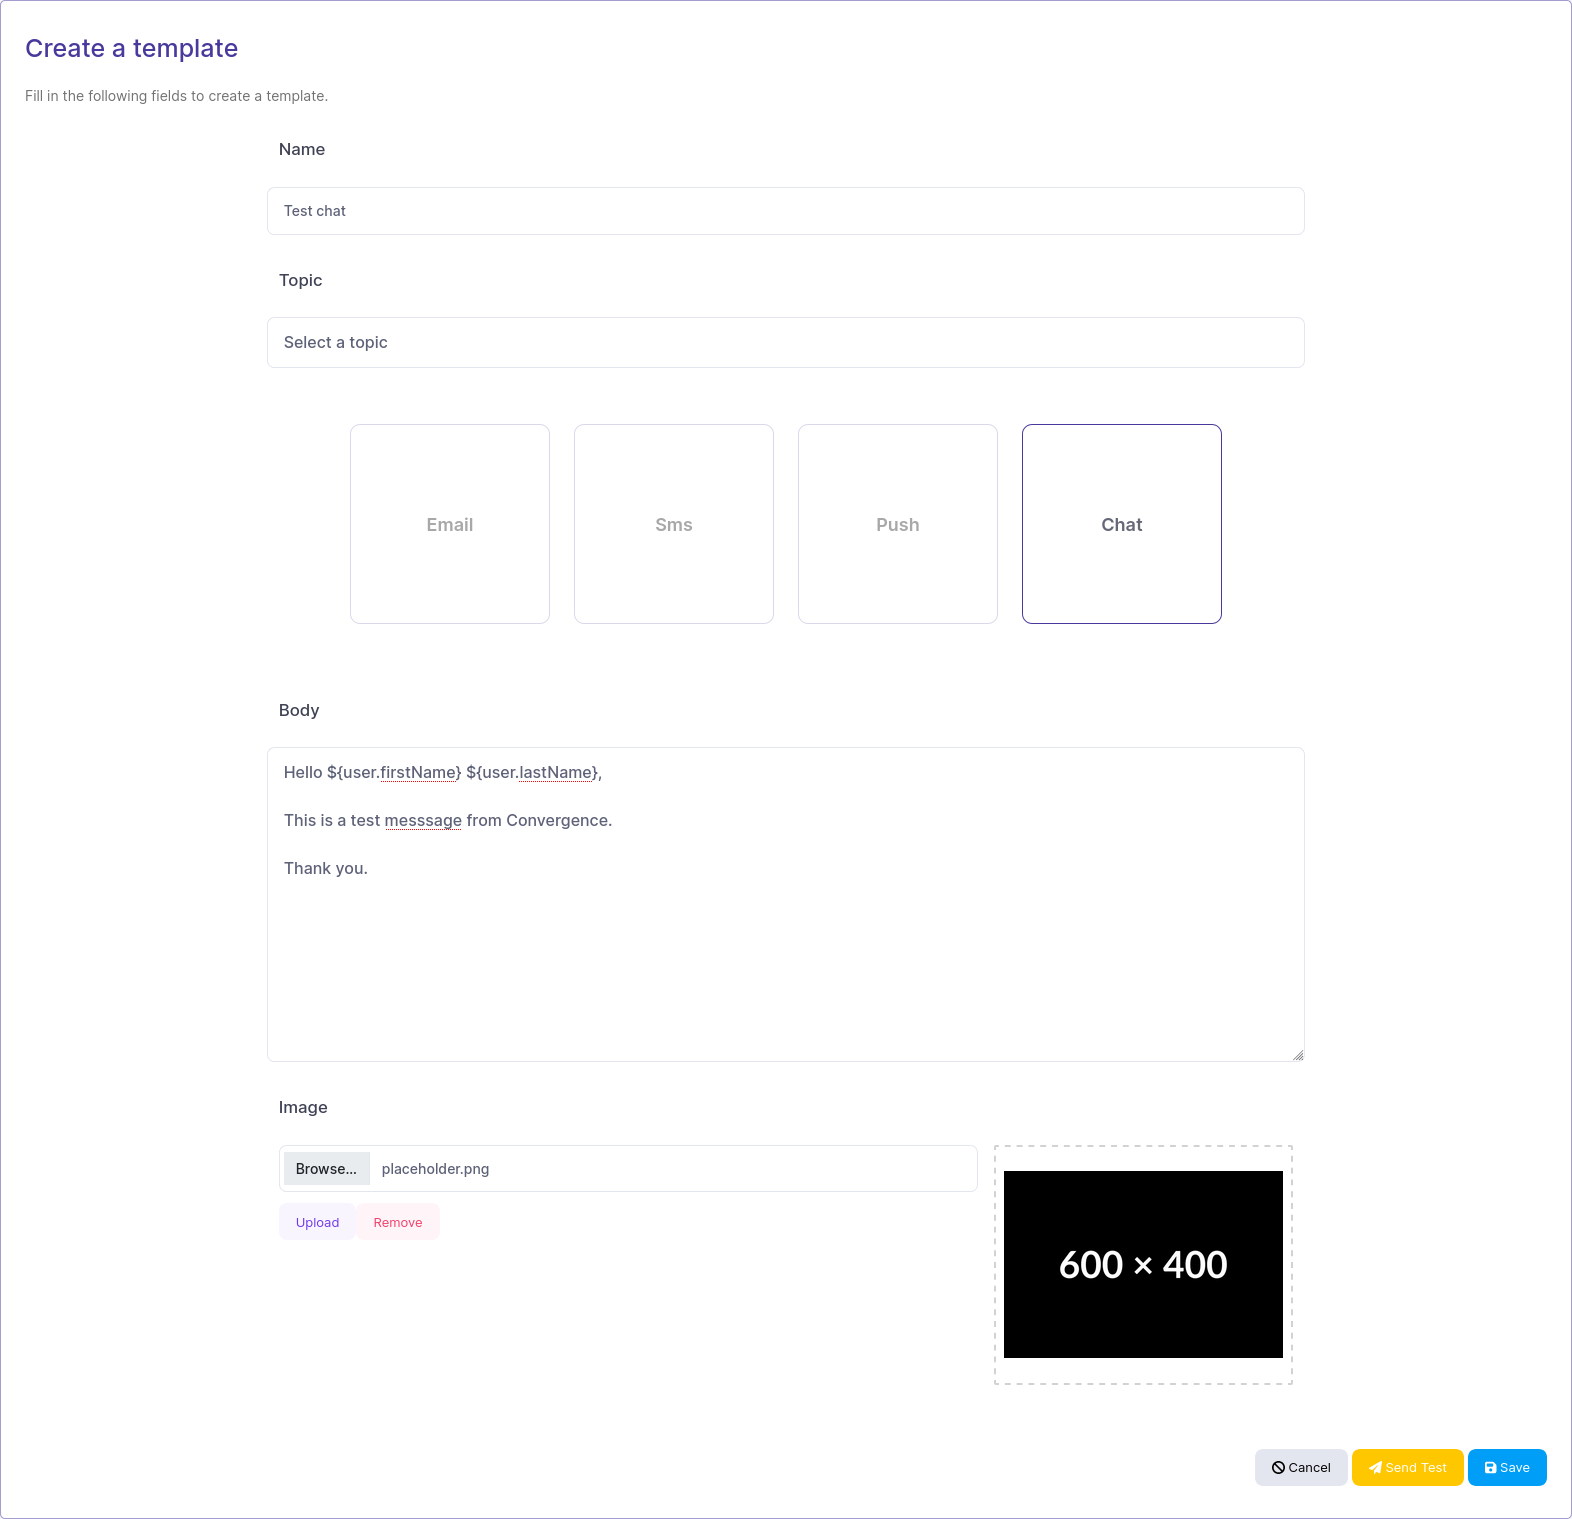
\includegraphics[width=\textwidth]{app/template1}
    \caption{Template creation page}
    \label{ss-template}
\end{figure}

\subsection{Triggers management}
Creating a notification trigger involves selecting a notification template and a target audience,
choosing a delivery type (one-time or recurring), and setting the associated parameters, including frequency,
start date, and end date.

The figure \ref{ss-create-trigger} shows the actual creation form where we selected an SMS test template,
all SMS subscribers audience, the one time delivery type, and chose the option to send immediately.
This option eliminates the need to specify a start date.

On saving success, the client navigates back to the notification triggers listing page, where we can
see our created at the top of the list, showing its important details. Notice the status of the trigger
is now set to "Running" while it is sending notifications. Upon acheiving, the status will change to "Complete"
as shown for the older triggers in the figure \ref{ss-triggers}.


\begin{figure}[hbt!]
    \centering
    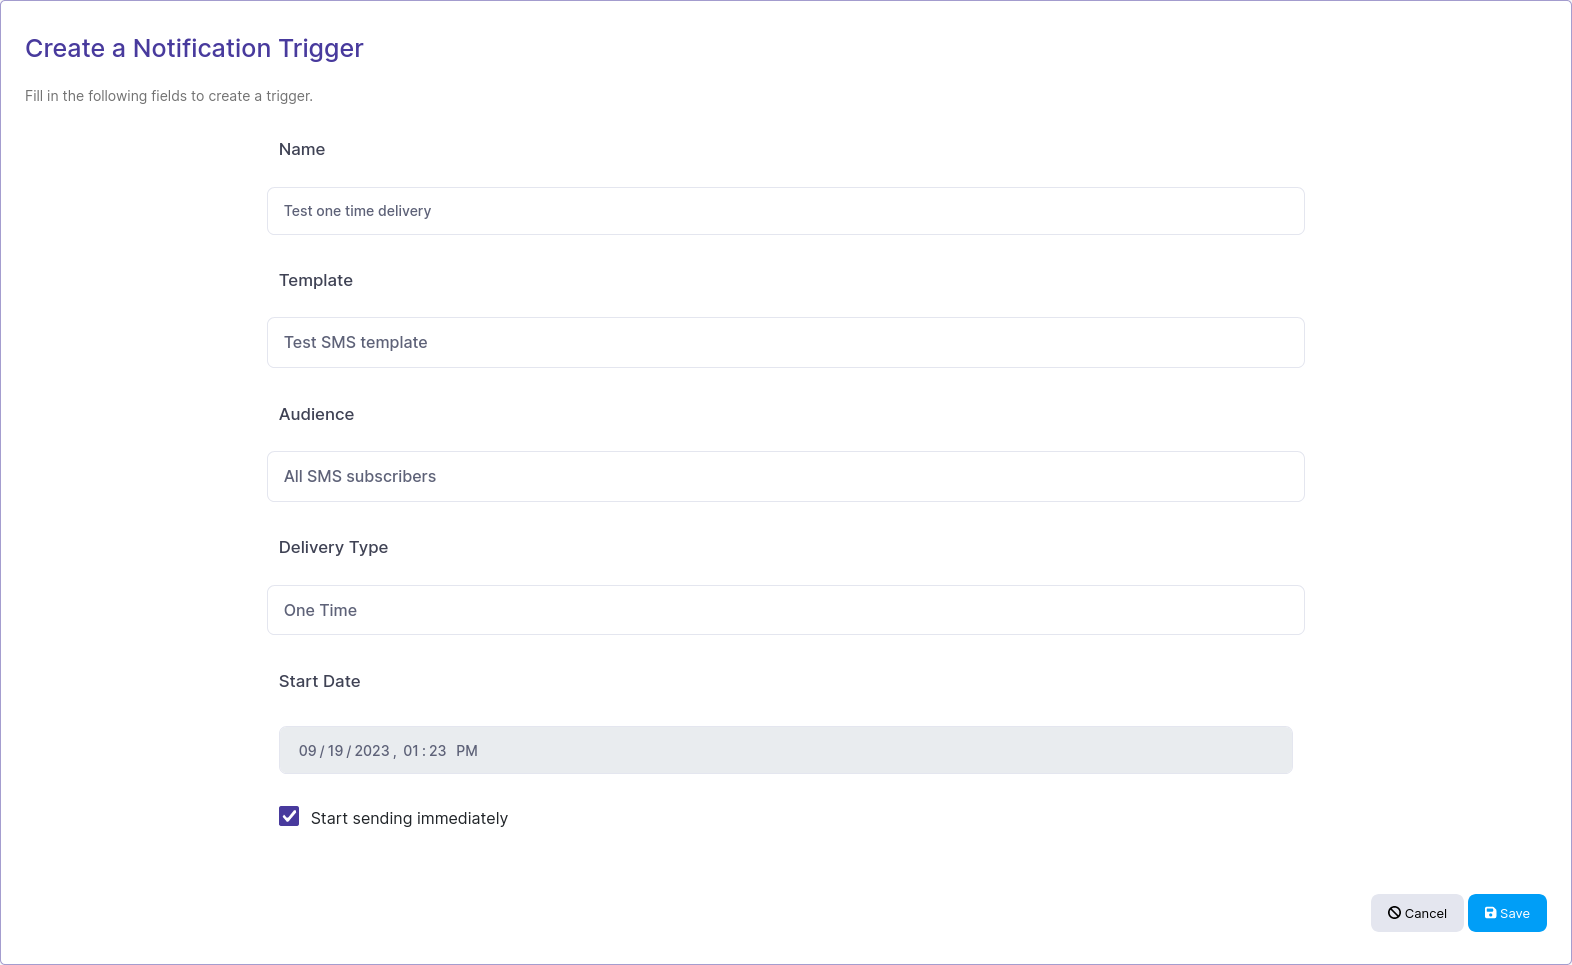
\includegraphics[width=\textwidth]{app/create-trigger}
    \caption{Trigger creation page}
    \label{ss-create-trigger}
\end{figure}

\begin{figure}[hbt!]
    \centering
    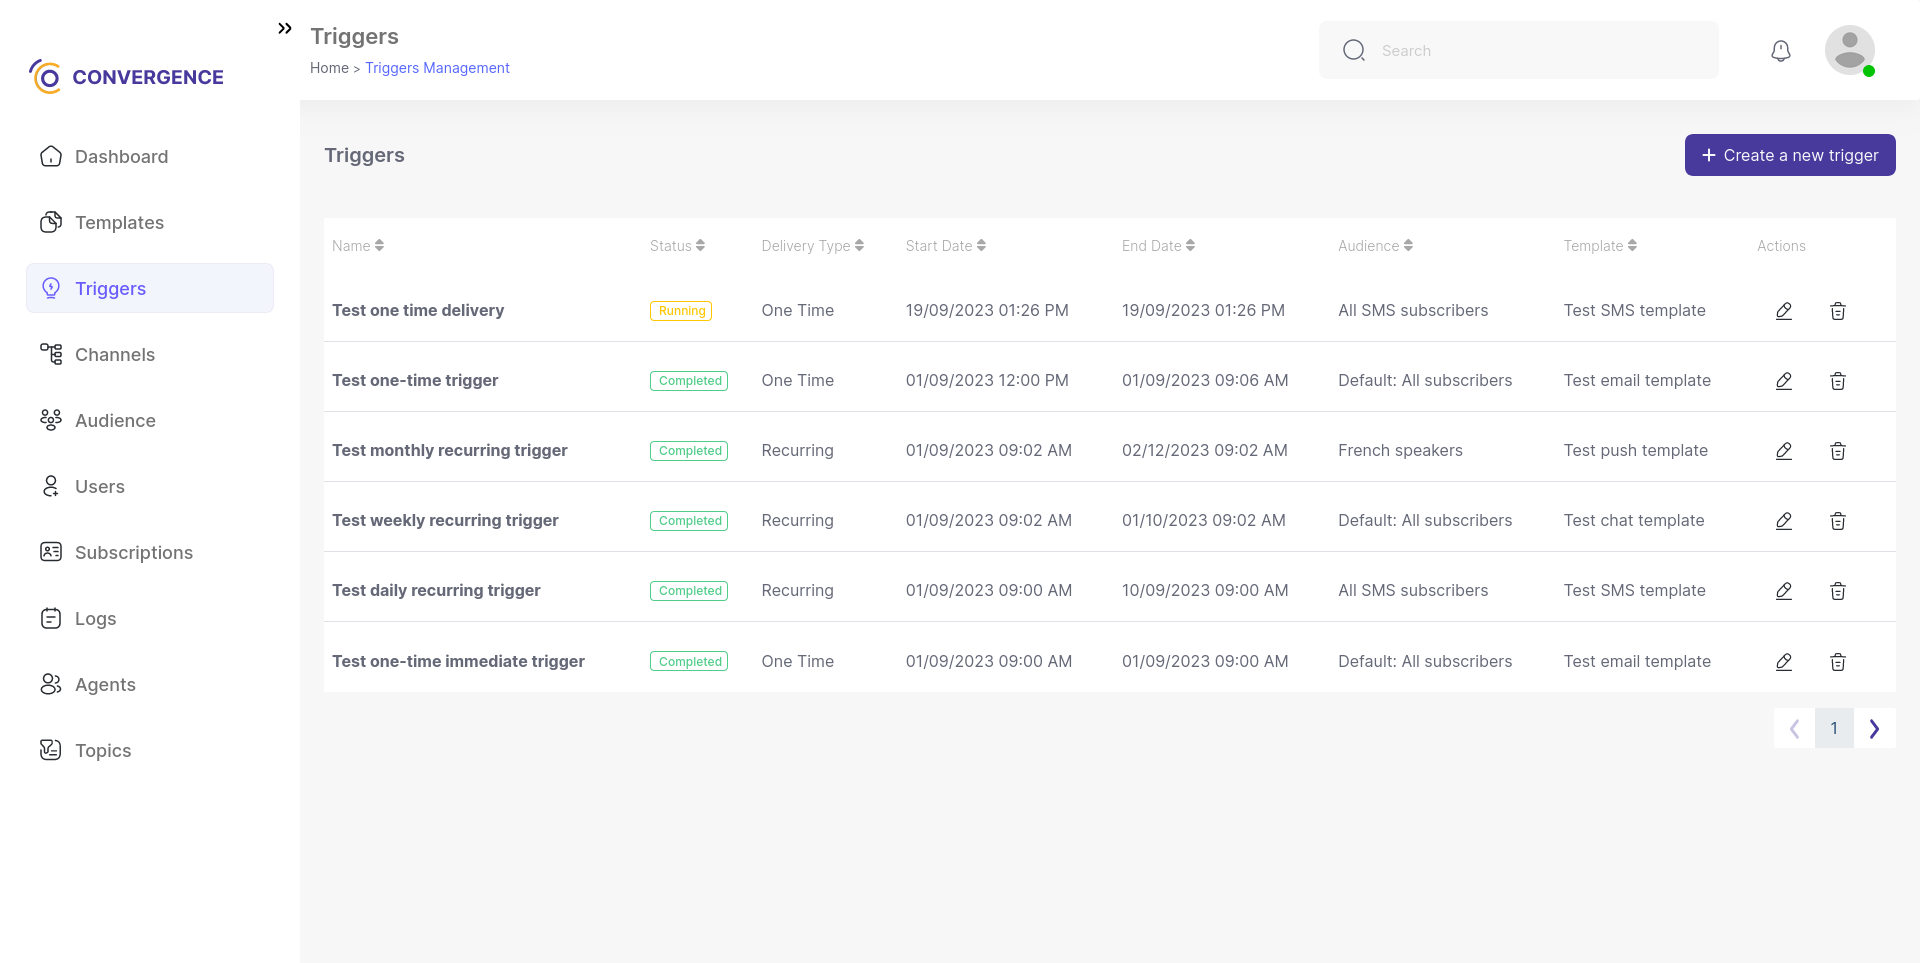
\includegraphics[width=\textwidth]{app/triggers}
    \caption{Triggers management page}
    \label{ss-triggers}
\end{figure}


\phantomsection
\section*{Conclusion}


\addcontentsline{toc}{section}{Conclusion}
In this chapter, we focused on the second release of our project, which centers around improving
the notification sending processs. We started by specifying requirements related to this release,
and delve into crucial design aspects to transform those requirements into actual implementations.
Finally, we highlight our progress by showcasing visual representations of features covering
templates and triggers management to enhance our notification system.